\section{集合大小与可加性}
\label{sec:meas-size-additivity}

测度要推广的是我们已经会做的几件事：数有限集合的元素，量区间的长度，算矩形的面积与体积。本节先从这些测量中提取共同的相加规则，再用有限个矩形从内外两侧逼近一般集合，得到Jordan测量。有理点集的例子将说明，只允许有限个矩形会给某些稀疏的集合不合理的大小；改用可数个区间后，问题转化为一项新的要求：测量规则要对可数运算封闭，并对可数分割可加。

\subsection{计数、长度与体积}
\label{sec:meas-count-length-volume}

\paragraph{计数与加权计数}
对有限集合$A$，用$\#A$表示它的元素个数。若$A$与$B$不相交，合并后每个元素恰好被数一次，所以$\#(A\cup B)=\#A+\#B$。更一般地，给有限集合$X$的每个点$x$配一个非负权重$w_x$，令$A\subseteq X$的大小为$\sum_{x\in A}w_x$。不相交集合合并时，大小仍是两部分之和。权重全取$1$时就是计数；权重不同时，它可以表示质量、费用或频率。

图~\ref{fig:meas-count-length}(a)中$X=\{1,2,3,4,5\}$，权重依次为$0.5,1,2,0.5,1$。分组$A=\{1,2,3\}$、$B=\{4,5\}$后，$A$有$3$个元素、总权重$3.5$，$B$有$2$个元素、总权重$1.5$。整体的个数$5=3+2$，总权重$5=3.5+1.5$。两种大小的数值不同，却遵守同一条规则：不交的部分相加得到整体。

\paragraph{区间长度与矩形体积}
实轴上的区间无法逐个数元素。对端点为$a\leq b$的区间，不论端点是否属于它，规定长度为$b-a$，记作$\ell$。在$\mathbb R^d$中，各边与坐标轴平行的\term{矩形}（rectangle）$R=I_1\times\cdots\times I_d$由$d$个区间相乘得到，规定它的体积为$\lvert R\rvert=\ell(I_1)\cdots\ell(I_d)$。$d=2$时这是面积，$d=1$时回到长度。

长度不是计数的推广。任意两个非退化区间都与$\mathbb R$等势，按元素个数无法区分$[0,1]$与$[0,2]$，长度却分别为$1$和$2$（等势的讨论可参考\BookChapterRef{chap:cardinality}{卷一第3章“基数”}）。所以计数与长度是两种不同的赋值：前者数元素，后者量集合在实轴上占据的范围。无限集合不能笼统地说“一样大”，要先说明用哪一种赋值。

\paragraph{有限个不交矩形的体积}
设$E$是有限个两两不交矩形$R_1,\dots,R_m$的并，自然规定$\lvert E\rvert=\sum_{k=1}^m\lvert R_k\rvert$。同一个$E$往往有多种拆法，这个定义要有意义，必须先说明结果与拆法无关。先看一维：一个区间被切点$a=t_0<t_1<\dots<t_r=b$分开后，小区间长度之和$\sum_j(t_j-t_{j-1})$逐项相消，等于$b-a$。

对两种拆法，取它们全部的端点，从小到大排列，就得到两种拆法的\emph{共同细分}。每种拆法中的每个区间都恰好是若干细分小区间之并，所以两种长度和都等于细分小区间的长度和。$d$维时，在每个坐标方向上取全部边的端点，得到一张网格；每个矩形是若干网格小块之并，体积等于这些小块体积之和，因为乘积$\prod_i\ell(I_i)$对每个因子的切分都可加。于是两种拆法给出同一个总体积。

图~\ref{fig:meas-count-length}(b)中$E=[0,2)\cup[3,4)$。第一种拆法为$[0,1.5),[1.5,2),[3,4)$，长度和为$1.5+0.5+1=3$；第二种为$[0,0.5),[0.5,2),[3,3.5),[3.5,4)$，长度和为$0.5+1.5+0.5+0.5=3$。共同细分的切点是$0,0.5,1.5,2,3,3.5,4$，两种拆法都由这些小区间拼成，总长度相同。

\begin{figure}[!htbp]
  \centering
  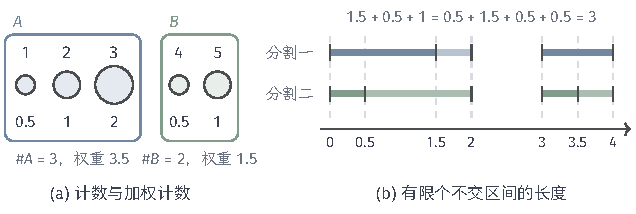
\includegraphics[width=107.6mm]{figures/02-abstract-mathematics/01-metric-and-measure/tikz/c2-count-length/figure.pdf}
  \caption{计数、加权计数与长度遵守同一条不交相加规则。(a)五个点按权重画成大小不同的圆，分成$A=\{1,2,3\}$与$B=\{4,5\}$后，个数$3+2=5$，总权重$3.5+1.5=5$；(b)集合$E=[0,2)\cup[3,4)$的两种不交区间分割，灰色竖线是共同细分的切点，两种分割的长度和都等于$3$。}
  \label{fig:meas-count-length}
\end{figure}

\paragraph{可数拆分时应保持的规则}
上面的可加性只涉及有限个矩形。分析中还会遇到可数拆分。例如
\[
 [0,1)=\bigcup_{k\geq1}\bigl[1-2^{1-k},\,1-2^{-k}\bigr),
\]
这些区间两两不交，长度依次为$\tfrac12,\tfrac14,\tfrac18,\dots$，级数和为$1$，恰好等于$[0,1)$的长度。我们希望这条规则对一切可数拆分都成立：整体长度等于各部分长度的级数和。这不能从有限可加性直接推出，因为有限个区间的拼接只能处理有限个部分。

规则也不能推广到任意多个部分。$[0,1]$是全部单点$\{x\}$之并，每个单点长度为$0$，而“$0$的不可数和”没有定义；若把它理解为$0$，就会得到$[0,1]$的长度为$0$的荒谬结论。所以“有限”与“可数”之间有一条要守住的界线：可数拆分应当保持可加，不可数拆分不作要求。后面建立的测度正是按这条界线设计的。

\subsection{Jordan测量}
\label{sec:meas-jordan}

有限个不交矩形的并只是很少一部分集合。对更一般的有界集合，自然的想法是从里面和外面同时用这类简单集合去逼近，卷二定义区域积分时用的正是这种方法（可参考\BookChapterRef{chap:region-integrals}{卷二第21章“区域积分”}）。下面把有限个有界矩形的并称为\term{初等集合}（elementary set）。它总能改写成有限个不交矩形的并，所以上一小节的体积对它有定义。

\paragraph{内外逼近}
初等集合的体积对包含关系单调。若初等集合$P\subseteq Q$，则$Q\setminus P$仍是初等集合，于是$\lvert P\rvert\leq\lvert P\rvert+\lvert Q\setminus P\rvert=\lvert Q\rvert$。由此可以比较任意一个内部逼近与任意一个外部逼近。

\begin{definition}[Jordan测量]
\label{def:meas-jordan}
设$E\subseteq\mathbb R^d$有界。称
\[
 \begin{aligned}
  J_*(E)&=\sup\{\lvert P\rvert:P\text{为初等集合},\ P\subseteq E\},\\
  J^*(E)&=\inf\{\lvert Q\rvert:Q\text{为初等集合},\ E\subseteq Q\}
 \end{aligned}
\]
分别为$E$的\term{Jordan内测量}（Jordan inner content）与\term{Jordan外测量}（Jordan outer content），其中空集作为初等集合体积为$0$。若$J_*(E)=J^*(E)$，称$E$是\term{Jordan可测}（Jordan measurable）的，公共值记为$J(E)$，称为$E$的\term{Jordan测量}（Jordan content）。
\end{definition}

任取内部初等集合$P\subseteq E$与外部初等集合$Q\supseteq E$，有$P\subseteq Q$，所以$\lvert P\rvert\leq\lvert Q\rvert$，从而总有$J_*(E)\leq J^*(E)$。Jordan可测的意思是两侧能夹逼到同一个数。

\paragraph{边界判据}
两侧逼近之差来自同时接触$E$与$E$外部的那些矩形，所以能否夹逼取决于边界。卷二证明了：有界集合$E$是Jordan可测的，当且仅当它的边界$\partial E$能被有限个总体积任意小的矩形覆盖。直观地说，取一张很细的网格，含于$E$的小块给出内部逼近，与$E$相交的小块给出外部逼近，两者只差与边界相交的小块。

这个判据把问题变成了一个覆盖问题：边界能否用有限个矩形以任意小的总体积盖住。圆盘、多边形等边界光滑或分段光滑的集合都满足它。下面两个一维例子分别说明有限覆盖能做到什么、做不到什么。

\paragraph{有限覆盖可以处理的无限集合}
取$E=\{1/n:n\geq1\}\subseteq\mathbb R$。它不含非退化区间，内测量为$0$。对任意正整数$N$与$\varepsilon>0$，用一个区间$[0,1/N]$盖住$n\geq N$的全部点，再用长度各为$\varepsilon/N$的小区间盖住$1,\tfrac12,\dots,\tfrac1{N-1}$。外部初等集合的总长度不超过$1/N+\varepsilon$，令$N\to\infty$、$\varepsilon\to0$得$J^*(E)=0$。

所以$E$是Jordan可测的，测量为$0$。这里要分清两种“有限”：$E$的元素有无限多个，用来逼近的区间却只有有限个。有限个区间能盖住无限多个点，前提是这些点聚集在少数位置附近；本例中它们聚向$0$，一个短区间就能接住几乎全部的点。

\paragraph{有理点集的反例}
取$E=\mathbb Q\cap[0,1]$。任何非退化区间都含无理数，所以含于$E$的初等集合只能由单点组成，$J_*(E)=0$。另一方面，设初等集合$Q\supseteq E$由区间$I_1,\dots,I_m$组成。把每个$I_k$换成闭包$\overline{I_k}$，长度不变，而$\bigcup_k\overline{I_k}$是含$E$的闭集。$E$在$[0,1]$中稠密，这个闭集必须含$[0,1]$，所以$\lvert Q\rvert\geq1$。$[0,1]$本身是外部初等集合，故$J^*(E)=1$。

内外测量分别为$0$与$1$，$E$不是Jordan可测的。问题出在有限覆盖：有理点到处都是，有限个区间要盖住它们，就不得不连同中间的全部无理数一起盖住。用边界判据看也是一样：$E$的边界是整个$[0,1]$，不能用总长度很小的有限个区间盖住。

\paragraph{改用可数覆盖}
如果允许可数个区间，情况完全不同。把$E$中的点排成一列$q_1,q_2,\dots$。给定$\varepsilon>0$，用长度为$\varepsilon2^{-k}$、以$q_k$为中心的开区间盖住$q_k$。这些区间盖住了$E$，长度总和为$\sum_{k\geq1}\varepsilon2^{-k}=\varepsilon$。图~\ref{fig:meas-jordan-rationals}对比了两种覆盖：有限覆盖必须铺满$[0,1]$，可数覆盖的区间越来越短，总长度可以任意小。在可数覆盖之下，有理点集的大小应当是$0$。

\begin{figure}[!htbp]
  \centering
  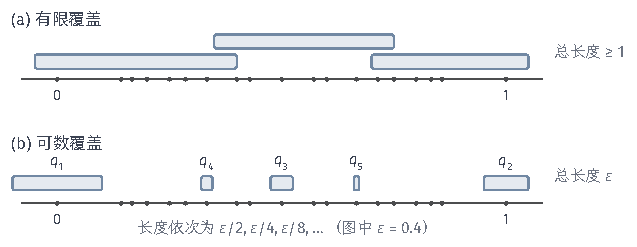
\includegraphics[width=107.8mm]{figures/02-abstract-mathematics/01-metric-and-measure/tikz/c2-jordan-rationals/figure.pdf}
  \caption{用区间覆盖$[0,1]$中的有理点。(a)有限个区间要盖住稠密的有理点，闭包后必须铺满$[0,1]$，总长度不小于$1$；(b)按排列顺序给第$k$个有理点$q_k$分配长度$\varepsilon2^{-k}$的区间，图中只画出前五个，长度依次减半，总长度为$\varepsilon$。}
  \label{fig:meas-jordan-rationals}
\end{figure}

\paragraph{需要重新建立的测量规则}
有理点集还暴露了Jordan测量的另一个缺陷。每个单点都Jordan可测且测量为$0$，它们的可数并$E$却不Jordan可测，所以Jordan可测集合族对可数并不封闭。而分析中处处需要可数运算：一列集合取并或取交，用逐步逼近得到的集合列求极限，把一个集合分成可数个部分。

由此提出两项要求。第一，允许测量的集合族应当对补集和可数并封闭，从而对可数交也封闭。第二，若一个集合被分成可数个不交的可测部分，整体的大小应等于各部分大小的级数和。注意我们没有要求“所有集合都可测”：第一项只规定集合族要有的封闭性，它究竟包含哪些集合，要在构造中确定。下一节先把这两项要求写成定义，满足它们并与长度一致的测量是否存在，由第~\ref{sec:meas-construction}节回答。
